\chapter{异常}

\section{异常}

\subsection{异常(Exception)}

异常就是程序在运行过程中出现的非正常的情况,它可以被捕获并处理,以防止程序崩溃。\\

exception是一个异常类,发生异常的时候会抛出一个异常对象。如果不处理异常,程序就会被中断。\\

\begin{table}[H]
    \centering
    \setlength{\tabcolsep}{5mm}{
        \begin{tabular}{|l|l|}
            \hline
            \textbf{异常}          & \textbf{描述}  \\
            \hline
            std::exception         & 所有异常的父类 \\
            \hline
            std::bad\_alloc        & 内存分配失败   \\
            \hline
            std::bad\_cast         & 类型转换失败   \\
            \hline
            std::logic\_error      & 逻辑错误       \\
            \hline
            std::invalid\_argument & 无效参数       \\
            \hline
            std::out\_of\_range    & 超出有效范围   \\
            \hline
            std::runtime\_error    & 运行时错误     \\
            \hline
            std::overflow\_error   & 发生上溢       \\
            \hline
            std::underflow\_error  & 发生下溢       \\
            \hline
        \end{tabular}
    }
    \caption{常用异常}
\end{table}

例如当数组访问越界时,会抛出一个std::out\_of\_range异常;当内存分配失败,会抛出一个std::bad\_alloc异常。\\

\subsection{捕获异常}

try-catch结构可以用于捕获并处理异常,将可能出现异常的代码放在try结构中,将异常处理的代码放在catch结构中。\\

当在try结构中出现异常时,程序会跳转到catch结构中,执行catch结构中的代码。一个异常被处理后,将不再影响程序的执行。\\

\begin{figure}[H]
    \centering
    
\includegraphics{img/Chapter11/11-1/1.png}
\end{figure}

what()是异常类提供的一个公共方法,它已被所有子异常类重载。\\

\mybox{内存分配失败}

\begin{lstlisting}[language=C++]
#include <iostream>
#include <exception>

using namespace std;

int main() {
    try {
        int *arr = new int[0xfffffffff];
        delete arr;
    } catch (bad_alloc &e) {
        cerr << e.what() << endl;
    }

    return 0;
}
\end{lstlisting}

\begin{tcolorbox}
    \mybox{运行结果}
    \begin{verbatim}
std::bad_alloc
	\end{verbatim}
\end{tcolorbox}

\vspace{0.5cm}

\subsection{throw}

throw关键字用于抛出一个异常。\\

\begin{figure}[H]
    \centering
    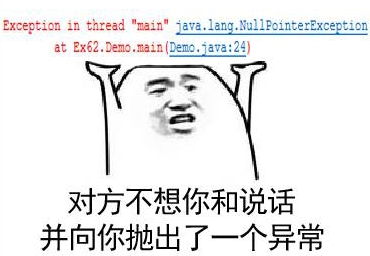
\includegraphics{img/Chapter11/11-1/2.png}
\end{figure}

\mybox{阶乘}

\begin{lstlisting}[language=C++]
#include <iostream>
#include <exception>

using namespace std;

int factorial(int n) {
    if (n < 0) {
        throw "Factorial of negative numbers is not defined.";
    }

    if (n == 0 || n == 1) {
        return 1;
    }
    return n * factorial(n - 1);
}

int main() {
    int n;
    cout << "Enter n: ";
    cin >> n;

    try {
        int fact = factorial(n);
        cout << n << "! = " << fact << endl;
    } catch (const char *e) {
        cerr << e << endl;
    }

    return 0;
}
\end{lstlisting}

\begin{tcolorbox}
    \mybox{运行结果}
    \begin{verbatim}
Enter n: -1
Factorial of negative numbers is not defined.
	\end{verbatim}
\end{tcolorbox}

\newpage

\section{自定义异常}

\subsection{自定义异常}

为了满足某些特定的需求,用户可以自定义异常,自定义异常继承于exception类或其子类。自定义异常的目的是为了提供更具体和有意义的错误处理。\\

\mybox{库存}

\begin{lstlisting}[language=C++]
#ifndef _OUT_OF_STOCK_EXCEPTION_H_
#define _OUT_OF_STOCK_EXCEPTION_H_

#include <string>
#include <exception>

class OutOfStockException : public std::exception {
    private:
    std::string msg;

    public:
    OutOfStockException(std::string msg);
    virtual const char *what() const noexcept override;
};

#endif
\end{lstlisting}

\begin{lstlisting}[language=C++]
#include "out_of_stock_exception.h"

OutOfStockException::OutOfStockException(std::string msg) {
    this->msg = msg;
}

const char *OutOfStockException::what() const noexcept {
    return msg.c_str();
}
\end{lstlisting}

\begin{lstlisting}[language=C++]
#ifndef _PRODUCT_H_
#define _PRODUCT_H_

#include <string>
#include "out_of_stock_exception.h"

class Product {
    private:
    std::string name;
    int stock;

    public:
    Product(std::string name, int stock);
    void purchase();
};

#endif
\end{lstlisting}

\begin{lstlisting}[language=C++]
#include "product.h"

Product::Product(std::string name, int stock) {
    this->name = name;
    this->stock = stock;
}

void Product::purchase() {
    if (stock == 0) {
        throw OutOfStockException(name + " is out of stock.");
    }
    stock--;
}
\end{lstlisting}

\begin{lstlisting}[language=C++]
#include <iostream>
#include "product.h"
#include "out_of_stock_exception.h"

using namespace std;

int main() {
    Product product("Cheeseburger", 50);

    try {
        for (int i = 0; i < 60; i++) {
            product.purchase();
        }
    } catch (OutOfStockException &e) {
        cerr << e.what() << endl;
    }

    return 0;
}
\end{lstlisting}

\begin{tcolorbox}
    \mybox{运行结果}
    \begin{verbatim}
Cheeseburger is out of stock.
	\end{verbatim}
\end{tcolorbox}

\newpage